
\documentclass[25pt, a1paper, portrait, margin=0mm, innermargin=15mm,
     blockverticalspace=15mm, colspace=15mm, subcolspace=8mm]{tikzposter}

\usepackage{amssymb,amsmath}
\usepackage{amsthm}
\usepackage{mathtools}

\usepackage{xcolor}
\usepackage{adjustbox}

\usepackage{tikz}
\usetikzlibrary{automata,arrows,positioning}

% core colours
\definecolor{brand-orange}{RGB}{255,121,0}

% support colours
\definecolor{brand-blue}{RGB}{75,180,230}

% functional greys
\definecolor{brand-lightgrey}{RGB}{246,246,246}

% functional colours
\definecolor{brand-func-blue}{RGB}{82,126,219}

\tikzstyle{switch-style}=[circle, draw, thin, fill=brand-blue, scale=0.3]
\tikzstyle{controller-style}=[rectangle, draw, thin, fill=brand-orange, scale=0.8]
\tikzstyle{rpath}=[ultra thick, brand-orange, opacity=0.4]

\theoremstyle{definition}
\newtheorem{theorem}{Theorem}
\theoremstyle{definition}
\newtheorem{definition}{Definition}
\theoremstyle{definition}
\newtheorem{lemma}{Lemma}

\title{Epidemic Control with Learning \& Optimization}
\author{Cristina Bazgan, Paul Beaujean, \'{E}ric Gourdin}
\institute{Universit\'{e} Paris-Dauphine, Orange Labs}
 
% Choose LAYOUT:  Default, Basic, Rays, Simple, Envelope, Wave, Board, Autumn, Desert,
\usetheme{Autumn}
\usecolorstyle[colorOne=brand-func-blue, colorTwo=brand-lightgrey,
colorThree=brand-blue]{Germany}

\begin{document}
\maketitle{}

\begin{columns}
  \column{0.3}
  \block{Context}{
    Malware spread, failure spread, systemic failure

  \begin{tikzfigure}[SDN Controller supervising its software-defined network]
      \begin{tikzpicture}[auto, thick]
       % Cloud creation
	\node[cloud, fill=gray!20, cloud puffs=16, cloud puff arc= 100,
	minimum width=7cm, minimum height=2.5cm, aspect=1] (cloud) at (0,0) {};
	\node (cloud-legend)[right=0.5cm of cloud] {Logical Topology};

       % Physical layer nodes
	\foreach \place/\x in {{(-2.5,0.3)/1}, {(-1.75,-0.55)/2},{(-1.2,0.55)/3},
	  {(-0.75,-0.7)/4}, {(-0.25,0)/5}, {(0.25,0.7)/6}, {(0.75,-0.3)/7}, 
	  {(1.5,0)/8},{(2.5,0.4)/9}}
	\node[switch-style] (a\x) at \place {};
       
	% SDN topology links
	\path[thin] (a1) edge (a2);
	\path[thin] (a1) edge (a3);
	\path[thin] (a2) edge (a3);
	\path[thin] (a3) edge (a6);
	\path[thin] (a2) edge (a4);
	\path[thin] (a5) edge (a6);
	\path[thin] (a5) edge (a4);
	\path[thin] (a5) edge (a2);
	\path[thin] (a5) edge (a7);
	\path[thin] (a6) edge (a7);
	\path[thin] (a6) edge (a9);
	\path[thin] (a6) edge (a8);
	\path[thin] (a8) edge (a9);
	\path[thin] (a7) edge (a8);
       
	\node[controller-style] (b)[above=3cm of a5] {};
	\node (b-legend)[right=1cm of b] {SDN Controller};
       
	\foreach \i in {1,...,9}
	  \path[rpath] (a\i) edge (b);
       
      \end{tikzpicture}
  \end{tikzfigure}
  }

  \column{0.7}
  \block{Model}{
    Inhomogeneous epidemics on undirected graphs.

    Markov chain representation.
    \begin{tikzfigure}[Markov chain]
      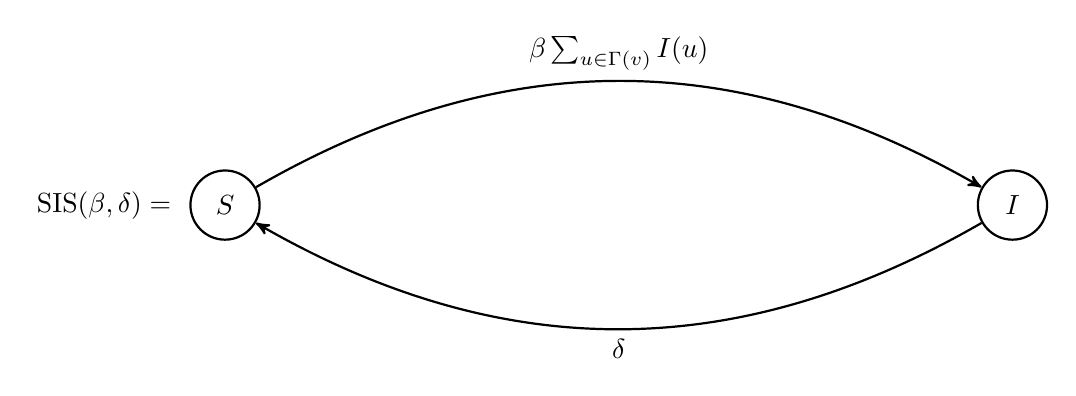
\begin{tikzpicture}[->, >=stealth', auto, thick, node distance=10cm]
      \tikzstyle{every state}=[fill=white, draw=black, thick, text=black, scale=1]

      \node[state] (S) {$S$};
      \node [left=0.1cm of S] {$\text{SIS}(\beta,\delta)=$};
      \node[state] (I)[right of=S] {$I$};

      \path (S) edge [bend left] node[above] {$\beta \sum_{u \in \Gamma(v)} I(u)$} (I);
      \path (I) edge [bend left] node[below] {$\delta$} (S);

      \end{tikzpicture}
    \end{tikzfigure}

    Cascading models.
  }
\end{columns}

\block{General framework}{
  \begin{tikzfigure}[]
      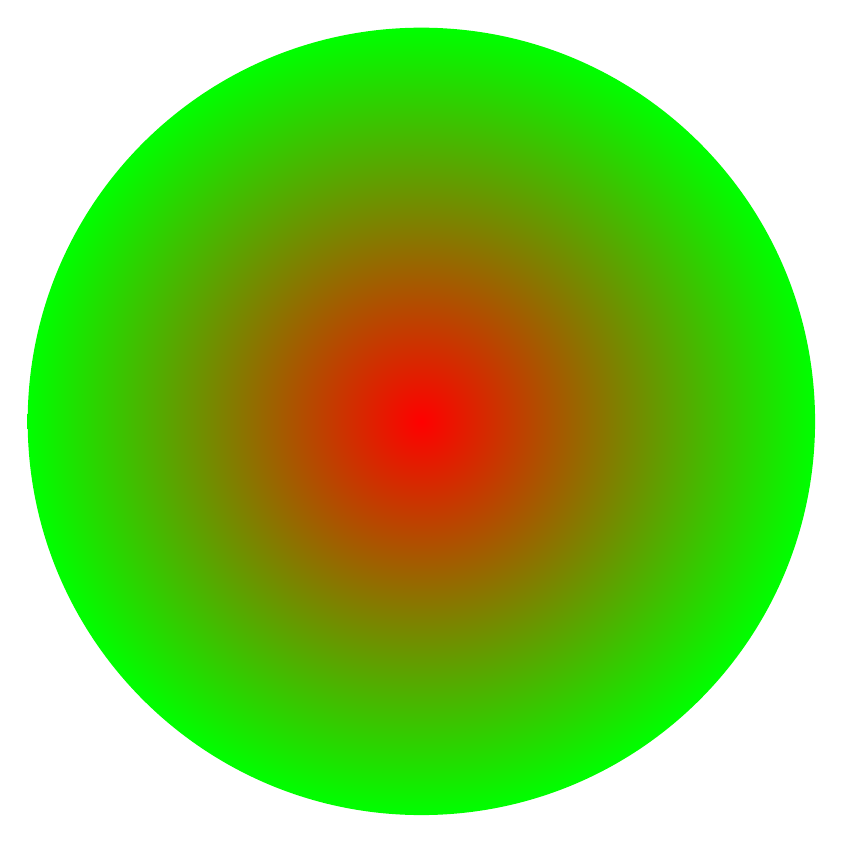
\begin{tikzpicture}
        \draw[draw=none,inner color=red, outer color=green] (0,0) circle (5cm);
      \end{tikzpicture}
  \end{tikzfigure}
}

\block{Learning the epidemic threshold}{

    \begin{minipage}[t]{0.6\textwidth}
    SDN Nodes running 1-class SVMs
    
    \begin{tikzfigure}[Closed walks of size $\log n$]
	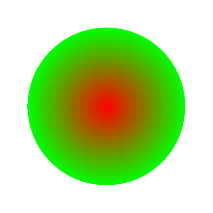
\begin{tikzpicture}
	  \draw[draw=none,inner color=red, outer color=green] (0,0) circle (1cm);
	\end{tikzpicture}
    \end{tikzfigure}
  \end{minipage}
  \begin{adjustbox}{valign=t}
      \begin{minipage}[t]{0.3\textwidth}
	SDN Controller running a parameter estimation algorithm

	\begin{tikzfigure}[Closed walks of size $\log n$]
	    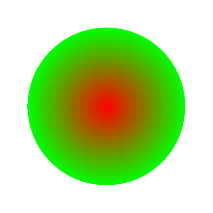
\begin{tikzpicture}
	      \draw[draw=none,inner color=red, outer color=green] (0,0) circle (1cm);
	    \end{tikzpicture}
	\end{tikzfigure}
      \end{minipage}
  \end{adjustbox}
}

\block{Optimizing the spectral radius}{

    \begin{minipage}[t]{0.3\textwidth}
    \begin{equation}
      \begin{split}
	\max & \sum_{e \in E} x_e\\
	  & A(x) \preceq t I\\
	  & x \in \{0,1\}^m
      \end{split}
    \end{equation}
    
  \end{minipage}
  \begin{adjustbox}{valign=t}
      \begin{minipage}[t]{0.7\textwidth}

	\innerblock{}{Combinatorics: subgraphs and closed walks
	  \begin{tikzfigure}[Closed walks of size $\log n$]
	      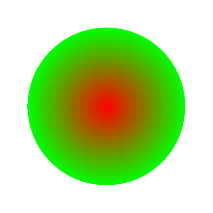
\begin{tikzpicture}
		\draw[draw=none,inner color=red, outer color=green] (0,0) circle (1cm);
	      \end{tikzpicture}
	  \end{tikzfigure}
	}
	\innerblock{}{Random Matrix Theory: randomized algorithms relying on concentration of measure
	  \begin{tikzfigure}[Wigner's semi-circle law]
	      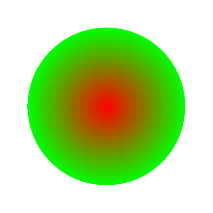
\begin{tikzpicture}
		\draw[draw=none,inner color=red, outer color=green] (0,0) circle (1cm);
	      \end{tikzpicture}
	  \end{tikzfigure}
	}
	\innerblock{}{Polynomials: real-stable polynomials and interlacing
	  families
	  \begin{tikzfigure}[Interlacing families]
	      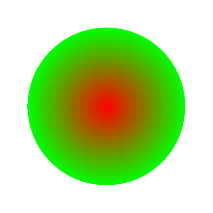
\begin{tikzpicture}
		\draw[draw=none,inner color=red, outer color=green] (0,0) circle (1cm);
	      \end{tikzpicture}
	  \end{tikzfigure}
	}
      \end{minipage}
  \end{adjustbox}
}

\end{document}
